% report.tex
% a report of the homework 2 - Computer Network 2016 Fall
\documentclass[12pt,a4paper]{extarticle}
\usepackage[margin=1in]{geometry}
\usepackage{xeCJK}
\usepackage{graphicx}
\usepackage{float}
\usepackage{subfig}
\usepackage{svg}

\setCJKmainfont{Noto Sans CJK TC}

\title{Computer Network\\ Homework 2 Report}
\author{林義聖\\B03902048}
\date{\today}

\begin{document}

\maketitle

\section{About the Program}

\subsection{Environment}

\begin{itemize}
	\item \textbf{Machine:} CSIE Workstation
	\item \textbf{GCC:} gcc 6.2.1 20160830
\end{itemize}

\subsection{Libraries}

I do this socket programming on Linux system and follow the newer official standard, which is POSIX Sockets API.

\section{How to Execute}

Simply type command ``\texttt{make}'', and then all the executable programs will be compiled.

There are totally 4 programs,
\begin{itemize}
	\item \texttt{sender}
	\item \texttt{receiver}
	\item \texttt{agent}
	\item \texttt{sender-mt}
\end{itemize}
And you can simply type commands like ``\texttt{./sender}'', and it will remind you the correct way to run the program.

\section{My Design}

\subsection{Program Structure}

\begin{figure}[H]
	\centering
	\subfloat[Sender] {
		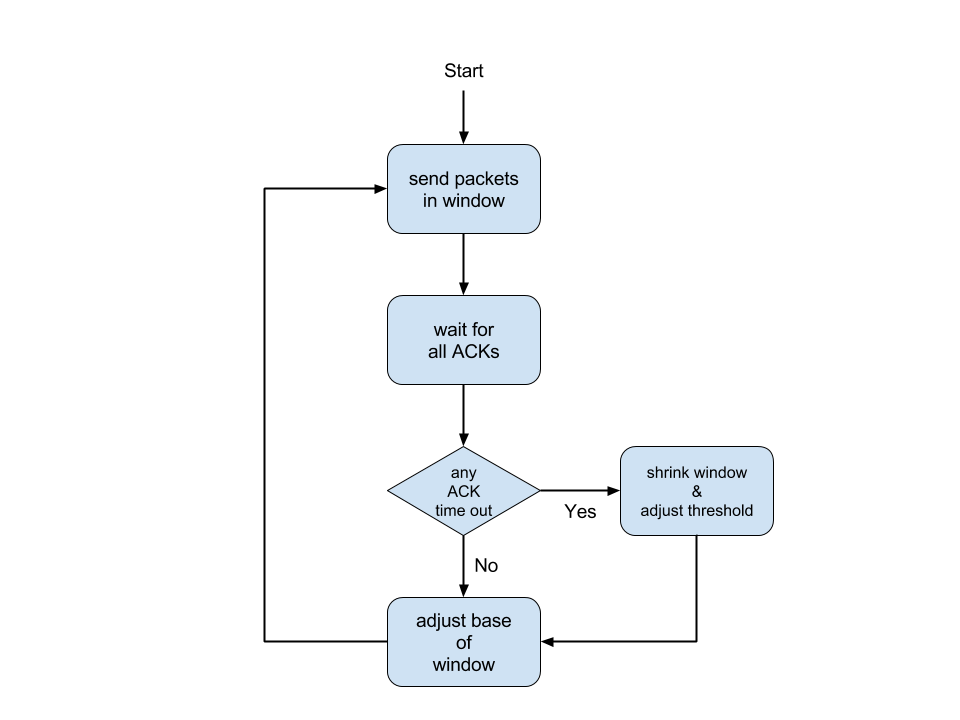
\includegraphics[width=0.45\linewidth]{sender.png}
	}
	\hfill
	\subfloat[Receiver] {
		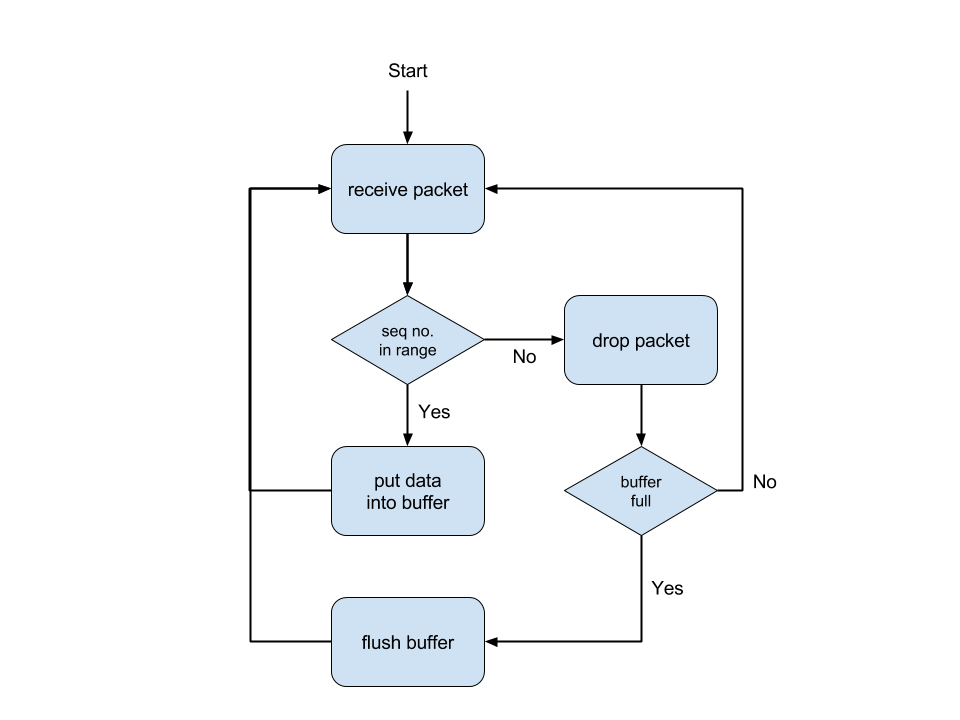
\includegraphics[width=0.45\linewidth]{receiver.png}
	}
	\caption{Simple Program Structure}
\end{figure}

\subsection{Difficulties and Solutions}

The difficulties I met in the homework assignment is how to design the program structure and how to combine the three programs: \texttt{sender}, \texttt{receiver}, and \texttt{agent}. It's really hard at the beginning that I had no idea where and how I can start. Latter, I tried to start these programs and make them communicate to each others through POSIX sockets. And I followed these steps to complete this assignment:
\begin{enumerate}
	\item Send packets from sender to agent, and forward them to receiver
	\item Send back ACK for each packet (Receiver)
	\item Send next packet only when receive ACK (Sender)
	\item Resend timeout packets (Sender)
	\item Randomly drop data packets (Agent)
	\item Add congestion control (Sender)
	\item Add buffer handling (Receiver)
\end{enumerate}

\subsection{Bonus}

I implemented a multi-agent sender. That is, there are many agents, and sender randomly pick one agent to send at each time it sends a packet.

\end{document}

